% THIS IS SIGPROC-SP.TEX - VERSION 3.1
% WORKS WITH V3.2SP OF ACM_PROC_ARTICLE-SP.CLS
% APRIL 2009
%
% It is an example file showing how to use the 'acm_proc_article-sp.cls' V3.2SP
% LaTeX2e document class file for Conference Proceedings submissions.
% ----------------------------------------------------------------------------------------------------------------
% This .tex file (and associated .cls V3.2SP) *DOES NOT* produce:
%       1) The Permission Statement
%       2) The Conference (location) Info information
%       3) The Copyright Line with ACM data
%       4) Page numbering
% ---------------------------------------------------------------------------------------------------------------
% It is an example which *does* use the .bib file (from which the .bbl file
% is produced).
% REMEMBER HOWEVER: After having produced the .bbl file,
% and prior to final submission,
% you need to 'insert'  your .bbl file into your source .tex file so as to provide
% ONE 'self-contained' source file.
%
% Questions regarding SIGS should be sent to
% Adrienne Griscti ---> griscti@acm.org
%
% Questions/suggestions regarding the guidelines, .tex and .cls files, etc. to
% Gerald Murray ---> murray@hq.acm.org
%
% For tracking purposes - this is V3.1SP - APRIL 2009

\documentclass{acm_proc_article-sp}
\usepackage{url}

%
\def\sharedaffiliation{%
\end{tabular}
\begin{tabular}{c}}
%

\begin{document}


\title{Similar Article Detection Using Locality Sensitive Hashing Technique on Wikipedia\titlenote{This effort is part of the CMSC828G, Data Intensive Computing with MapReduce, class project.}}
%
% You need the command \numberofauthors to handle the 'placement
% and alignment' of the authors beneath the title.
%
% For aesthetic reasons, we recommend 'three authors at a time'
% i.e. three 'name/affiliation blocks' be placed beneath the title.
%
% NOTE: You are NOT restricted in how many 'rows' of
% "name/affiliations" may appear. We just ask that you restrict
% the number of 'columns' to three.
%
% Because of the available 'opening page real-estate'
% we ask you to refrain from putting more than six authors
% (two rows with three columns) beneath the article title.
% More than six makes the first-page appear very cluttered indeed.
%
% Use the \alignauthor commands to handle the names
% and affiliations for an 'aesthetic maximum' of six authors.
% Add names, affiliations, addresses for
% the seventh etc. author(s) as the argument for the
% \additionalauthors command.
% These 'additional authors' will be output/set for you
% without further effort on your part as the last section in
% the body of your article BEFORE References or any Appendices.

\numberofauthors{5} %  in this sample file, there are a *total*
% of EIGHT authors. SIX appear on the 'first-page' (for formatting
% reasons) and the remaining two appear in the \additionalauthors section.
%
\author{
% You can go ahead and credit any number of authors here,
% e.g. one 'row of three' or two rows (consisting of one row of three
% and a second row of one, two or three).
%
% The command \alignauthor (no curly braces needed) should
% precede each author name, affiliation/snail-mail address and
% e-mail address. Additionally, tag each line of
% affiliation/address with \affaddr, and tag the
% e-mail address with \email.
%
% 1st. author
\alignauthor Samet Ayhan\\
       \affaddr{University of Maryland, Department of Computer Science}\\
       \affaddr{College Park, Maryland 20740}\\
       \email{sayhan@cs.umd.edu}
% 2nd. author
\alignauthor Joshua Bradley\\
       \affaddr{University of Maryland, Department of Computer Science}\\
       \affaddr{College Park, Maryland 20740}\\
       \email{jgbradley@cs.umd.edu}
% 3rd. author
\alignauthor Sarah Weissman\\
       \affaddr{University of Maryland, College of Information Studies}\\
       \affaddr{College Park, Maryland 20740}\\
       \email{sew@umd.edu}
}
% There's nothing stopping you putting the seventh, eighth, etc.
% author on the opening page (as the 'third row') but we ask,
% for aesthetic reasons that you place these 'additional authors'
% in the \additional authors block, viz.

\date{19 April 2013}
% Just remember to make sure that the TOTAL number of authors
% is the number that will appear on the first page PLUS the
% number that will appear in the \additionalauthors section.


\maketitle
\begin{abstract}
The growth of Internet has enabled collaboration and cooperation on a large scale, resulting in an abundant number of near-duplicate web documents. The range of occurrences is even more evident within Wikipedia articles, due to its editing largely being open. Except for particularly sensitive and/or vandalism-prone pages that are "protected" to some degree from editing, the reader of an article can edit the text by copying from another article without needing approval. Although we are not inspired to measure the quality of Wikipedia articles, we are interested in finding near-duplicate occurrences at various granularity levels. 

In this paper, we describe a novel similarity detection algorithm that utilizes locality sensitive hashing (LSH) technique on MapReduce framework. The algorithm has been designed and implemented to detect similar articles using large Wikipedia dumps, in compressed or uncompressed forms. Experimental results appear to support that our method is able to efficiently and effectively detect similar articles from large Wikipedia dumps.
\end{abstract}

% A category with the (minimum) three required fields
\category{H.3.3}{Information Storage and Retrieval}[Information Search and Retrieval]

\terms{Algorithms, Design, Performance}

\section{Introduction}
The online encyclopedia Wikipedia is a multilingual, free resource with its 26 million articles. All these articles with over 4.2 million in the English Wikipedia alone, are written collaboratively by volunteers around the world. Almost all of its articles can be edited by anyone with access to the site, and it has about 100,000 active contributors. In light of these facts, it is clear that unprecedented example of such a large-scale collaboration may result in duplicate or near duplicate articles in relatively granular level such as at sentence or multi-gram granularity \cite{wiki:weblink}

Furthermore, Wikipedia has a history of generating controversy over editorial quality and factual correctness. Although some studies have found Wikipedia’s accuracy to rival that of traditional encyclopedias, other studies have found numerous factual errors. Since Wikipedia may be edited anonymously, information is often freely copied between web sources or other Wikipedia articles. Additionally, many articles in Wikipedia lack citations. There is little mechanism for detecting and correcting such errors. One potential source of error on Wikipedia is factual information that varies over time and is not updated. Wilkinson found that the distribution of article edits has a long tail, meaning that a small number of articles have many edits while most articles have few, and that number of edits is directly related to article quality. Articles with low edits, and low editorial attention, are less likely to be updated when new information becomes available \cite{wilkinson:wiki}.

As a step toward identifying factual errors, we investigated the problem of finding near duplicate sentences on Wikipedia. Such near duplicate sentences may reflect factual information that has been updated in one article and not another, or merely inconsistencies that should be flagged and addressed. 

In order to come up with a novel algorithm that would allow us to detect near duplicate Wikipedia articles, we decided that we needed to answer the following questions, first:
\begin{itemize}
\item What is the most appropriate LSH technique to apply? Edit distance seems like a reasonable metric for near duplicate sentences, but no LSH family for edit distance is known to exist.
\item Compare different sentence similarity techniques for effectiveness. 
\item What is the appropriate granularity for analysis? Is comparing multiple consecutive sentences more effective than comparing single sentences? Similarly, what is the best shingle size?
\item How well do techniques for detecting near duplicate documents work when applied at the sentence level?
\item Do near duplicate sentences correspond to factual errors? Can these errors be automatically flagged or corrections suggested?
\end{itemize}

Along with these questions, we also considered the scalability and efficiency issues due to large size of Wikipedia dumps. To address these issues, we used the MapReduce computing framework and LSH techniques to group sentences with the same signatures and identify near duplicates.

The rest of this paper is organized as follows: In Section 2, we present related work, in Section 3, we explain the algorithm utilizing locality sensitive hashing, in Section 4, we present the working application within MapReduce framework. In Section 5, we discuss our experiments with various Wikipedia datasets. The final section contains concluding remarks and future work.

\section{Related Work}
A number of techniques have been implemented to identify similarity between documents in the literature. These techniques usually differ in terms of corpus of interest, signature representing the document, feature-set determined by the system, and the end goal. In addition to these differences, one can also consider the efficiency and scalability of the system, overall. 

In this section, we will go over some of theses techniques offered in the literature. Additionally, we will highlight our novel contribution.

Broder et al. introduced shingling to compute document similarity and containment. They also presented methods for using a subset of shingles while still allowing similarity and containment computations \cite{broder:resemblance}.

Seo et al. defined a general framework for text reuse detection. They introduced Discrete Cosine Transform (DCT) fingerprinting for general or local text reuse detection with high accuracy and efficiency \cite{seo:dct}.

Zhang et al. presented partial duplicate detection algorithm using sequence matching that transforms partial-duplicate detection task into three MapReduce jobs: 1.Indexing, 2.Sequence Duplicate Detection, 3.Sequence Matching \cite{zhang:pdc}.

Hajishirzi et al. introduced an adaptive near-duplicate detection (ANDD) method by extending term-weighting framework to learn k-gram vectors. Provided that each document was represented by an informative real k-gram vector, similarity measures were computed to come up with predicted values of near-duplicates \cite{hajishirzi:andd}.

Lin described three MapReduce algorithms for computing pairwise similarity on document collections: 1.Based on brute force, 2.Treated as large-scale ad hoc retrieval, 3.Based on Cartesian product of postings lists \cite{lin:brute}.

Manku et al. used Charikar's fingerprinting technique for developing near-duplicate detection system. They presented an algorithmic technique for identifying existing f-bit fingerprints that differ from a given fingerprint in at most k bit-positions, for small k. They demonstrated that their system is useful not only for batch but also for online processing \cite{manku:web}.

Bendersky et al. examined two information flow representations: the timeline and the link graph. They proposed several simple unsupervised techniques for timeline construction link graph analysis \cite{bendersky:timeline}.

In order to handle large Wikipedia dumps with the order of tens or hundreds of gigabytes and even a few terabytes, we used MapReduce framework in this work, that was introduced by Dean and Ghemawat \cite{dean:mapreduce}. The implementation is able to stream the compressed bz2 dumps and feed into mappers and reducers for further processing, which will be detailed in the following sections.

\section{Algorithm Utilizing Locality Sensitive Hashing}

In this section, we introduce the algorithm that utilizes the locality sensitive hashing.

In order to measure document similarity we use a common LSH technique known as minhashing \cite{}. A minhash signature on a text document is calculated using a parametrized family of hash functions $F_i$, $1 \le i \le N$. In our case input documents are sentences. Each sentence is broken up into n-gram ``shingles''. For each shingle set $S$ we calculate $\{min_{s \in S}(F_i(s)\}$, the set of minimum hashes over the hash family. The signature on a document d is a vector of $K$ minhashes from the set of minimum hashes. In order to minimize false negatives we apply the technique sometimes known as ``banding'' \cite{Ullman} where multiple signatures are produced for each input document.

\subsection{Design}
Since signature techniques such as LSH are easily parallelized we designed our algorithm around the MapReduce framework. 

Describe MapReduce.

Because the minhash technique is parametrized by several values, including shingle length, signature vector size and number of signatures calculated, these values can also be considered as inputs for the MapReduce algorithm.

\begin{table}
MapReduce pseudocode:
\begin{verbatim}
initialize(){
 # configure and set up algorithm parameters
 # F = hash family;
 # L = shingle length;
 # K = vector length;
 # N = number of signatures to emit;
}

map(docid d, wikipage p){
  int sentence ct = 0;
  while s = nextSentence(p){
    shingles = shingleSet(s,L);
    minhashes = new List(|F|);
    for i = 1 ... |F|:
      minhashes[i] = Infinity;
    for g in shingles:
      for i = 1 ... |F|:
        minhashes[i] = min(F_i(g),minhashes[i]);
    for i = 1 ... N:
      sig = select(K, minhahses);
      emit(sig,(docid,sentencect));
    sentencect++;
  }
}
\end{verbatim}

\begin{verbatim}
reduce(signature sig, sentenceids [(d1,s1),(d2,s2) ...]){
  if [[(d1,s1),(d2,s2) ... ]| > 1:
    emit(sig, [(d1,s1), (d2,s2), ...]);
}
\end{verbatim}
\end{table}

\subsection{Implementation Details}

Our implementation is built on top of the Apache Hadoop MapReduce framework, using utilities from the Cloud9 library for parsing Wikipedia page text from the Wikipedia XML dump format. Sentences are parsed out over each document using a regular expression. Sentences that are too large or too small are discarded. The family of hash functions is implemented using a ``Multiply Shift''  \cite{} hashing scheme and is generated from a random seed using the Java Random class. The hash family is also parametrized by hash output key size and this value can be configured to affect the size of the output signatures.

\section{Working Application}
We explain the working application here...

\begin{figure}
\centering
\epsfig{file=figure1.eps,height=1in,width=2.2in}
\caption{Workflow within MapReduce Framework.}
\end{figure}

\section{Parameter Tuning}

As mentioned above the minhash algorithm is parametrized by several values, including shingle length, length of hash vectors, number of hash bands, and hash output size. Each of these parameters has an impact on the error rates in the minhash output. 

\subsection{Jaccard Similarity and Edit Distance}

Jaccard similarity is a measure of set similarity while our stated goal is to find sentences in Wikipedia that have been copied from one article to another and possibly edited. A more natural measure to use for this application is edit distance. There is no known locality sensitive hashing family for edit distance \citation{}.

In order to estimate Jaccard similarity of sentences $X$ and $Y$ in terms of edit distance we assume that $X$ and $Y$ are both of length $N$ and that their shingle sets are of maximum size (i.e. all shingles are unique). Also assume that $X$ and $Y$ have edit distance $e$.  Additionally, to simplify our calculations, we assume that edits are localized so that no shingle overlaps more than one edit.

(WLOG) Let $S$ be the set of shingles for X and let $S_o$ be the set of shingles of X that overlap edits. The maximum number of unique shingles for a sentence of length $N$ is $N - L + 1 = |S|$. Also, we can see that $e \le |S_o| \le e + L - 1$. Since edits at the start or end of the sentence will overlap with fewer shingles than edit mid-sentence.

Now we can define $|X \cup Y|$ and $|X \cap Y|$ in terms $S$ and $S_o$ as follows:
\begin{eqnarray*}
|X \cap Y| & = & |S| - |S_o| \\
|X \cup Y| & = & 2*|S_o| + |X \cap Y| \\
           & = & |S_o| + |S|
\end{eqnarray*}

Plugging in the values above for $|S_o|$ and $|S|$ we get:

\begin{eqnarray*}
E + N - L + 1  \le & |X \cup Y| & \le E + N \\
N - L + 1 - E  \ge & |X \cap Y| & \ge N - 2L - E + 2 \\
\end{eqnarray*}
\begin{eqnarray*}
\frac{N - L - E + 1 }{N - L + e + 1} >= & J(X,Y) & >= \frac{N - 2L - E + 2}{N + E}
\end{eqnarray*}

Note that, at least under this set of assumptions, the Jaccard similarity is always less than the ``edit similarity'' (1 - normalized edit distance):

\begin{eqnarray*}
J(X,Y) & <= & \frac{N - E}{E + N - L + 1} - \frac{L - 1}{E + N - L + 1} \\
       & <= & \frac{N - E}{N} \\ 
       & =  & 1 - \frac{E}{N}
\end{eqnarray*}

Finally we can divide through the equations for J(X,Y) by N, which gives us:

\begin{eqnarray*}
\frac{1 - l - e}{1 - l + e} >= J(X,Y) >= \frac{1 - 2l - e}{1 + e}
\end{eqnarray*}

where $l$ is relative shingle size and $e$ is normalized edit distance.

Note that as relative shingle size goes to 0 there is a nice convergence for Jaccard similarity:
\[\lim_{l->0}J(X,Y) = \frac{1 - e}{1 + e}\]

\begin{figure*}
\centering
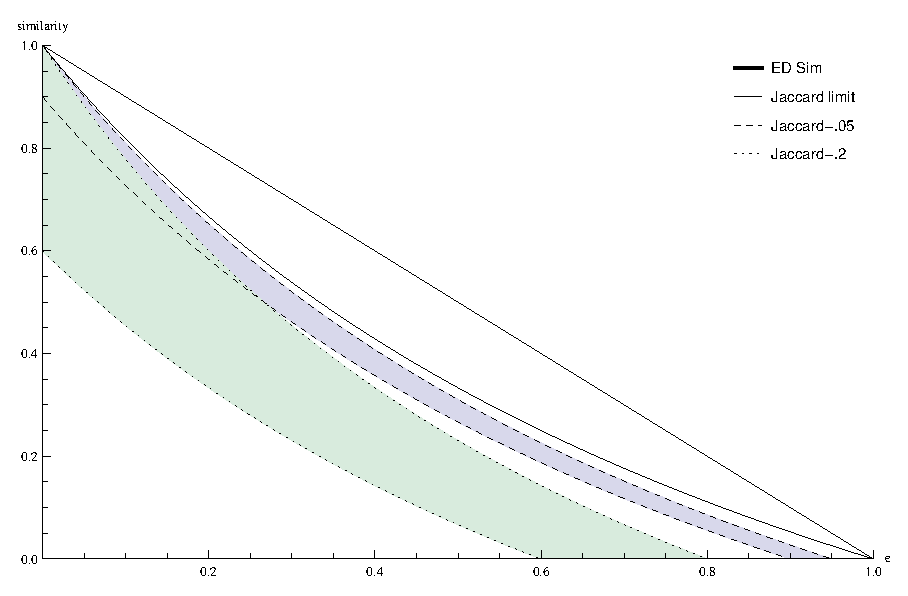
\epsfig{file=jac-ed-chart.eps,height=4in,width=6in}
\caption{Jaccard Similarity vs. normalized edit distance.}
\label{jac-ed}
\end{figure*}

As we would expect, Jaccard similarity decreases as edit distance increases, but it also decreases as shingle length increases. Figure \ref{fig:jac-ed} shows Jaccard Similarity plotted against edit distance for $l = .05$ and $l = .2$. At $l = .05$ and $e = .2$ our estimate for Jaccard similarity has already fallen to the range [0.58,0.65]. Clearly setting $l$ too high can increase the false positive rate, but setting $l$ too low will increase the false positive rate, since it will increase the size of the intersection of the shingle sets.

\subsection{False positives}

\begin{figure*}
\centering
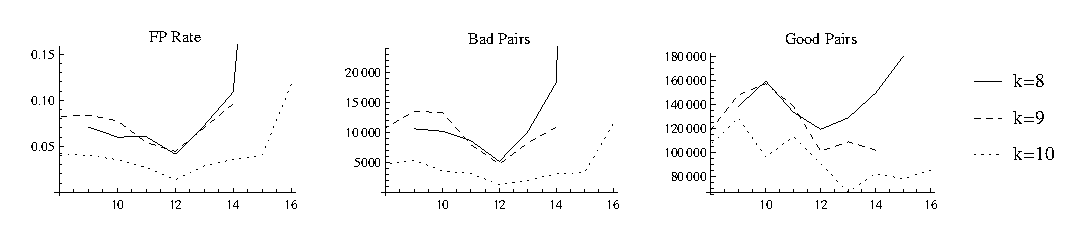
\epsfig{file=edgrid.eps,width=7in}
\caption{}
\label{ed-grid}
\end{figure*}


\section{Experiments and Discussion}
In this section, we discuss some of the issues we encountered regarding data representation, and archived data loading. We also present the performance optimizations we realized.

\subsection{Optimization}

We explain optimizations here...

\subsubsection{Optimization1}

An optimization we realized...

\subsubsection{Optimization-2}
Another optimization we realized...

\begin{figure*}
\centering
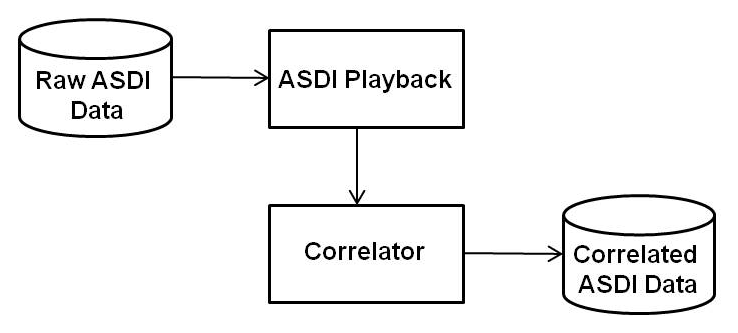
\epsfig{file=figure2.eps,height=1.5in,width=7in}
\caption{Some figure.}
\end{figure*}

Illustrated in Figure 2, explain the figure here...

\section{Conclusion and Future Work}
This paper presents our work on near-duplicate detection of Wikipedia articles at various granularity levels using LSH technique. Our novel MapReduce algorithm tackles the problem by transforming it into more manageable pieces where each piece handled in parallel. Our unique contribution includes empirical analysis of signatures belonging to Wikipedia articles at k-gram level. Experimental results verify that the proposed method is able to effectively and efficiently detect similar articles.

In the future, we would like to investigate revision histories of these articles, correlate them with their timestamps, and better relate similarities based on temporal dimensions. 

\section{Acknowledgments}
We would like to thank all of the anonymous contributors. We would especially like to thank Jimmy Lin for his advise and directions.

%
% The following two commands are all you need in the
% initial runs of your .tex file to
% produce the bibliography for the citations in your paper.
\bibliographystyle{abbrv}
\bibliography{sigproc}  % sigproc.bib is the name of the Bibliography in this case
% You must have a proper ".bib" file
%  and remember to run:
% latex bibtex latex latex
% to resolve all references
%
% ACM needs 'a single self-contained file'!
%
%APPENDICES are optional
%\balancecolumns
\balancecolumns
% That's all folks!
\end{document}
